\documentclass[12pt, twoside]{article}
\usepackage[letterpaper, margin=1in, head=30pt, headsep=0.1in]{geometry}
\usepackage[english]{babel}
\usepackage[utf8]{inputenc}
\usepackage{amsmath}
\usepackage{amsfonts}
\usepackage{amssymb}
\usepackage{tikz}
\usepackage{yhmath} %arcs using \wideparen{}
\usetikzlibrary{quotes, angles}

\usepackage{graphicx}
\usepackage{enumitem}
\usepackage{multicol}

%\usepackage{pgfplots}
%\pgfplotsset{width=10cm,compat=1.9}
%\usepgfplotslibrary{statistics}
%\usepackage{pgfplotstable}
%\usepackage{tkz-fct}
%\usepackage{venndiagram}

\usepackage{fancyhdr}
\pagestyle{fancy}
\fancyhf{}
\renewcommand{\headrulewidth}{0pt} % disable the underline of the header
\raggedbottom
\newif\ifmeta
\metatrue %print standards and topics tags

\title{High School Geometry problem sets}
\author{Chris Huson}
\date{April 2021}

%\fancyhead[RE]{\thepage}
%\fancyhead[RO]{\thepage \\ Name: \hspace{3cm}}
%\fancyhead[L]{BECA / Dr. Huson / 10th Grade Geometry\\* 7 June 2019}
%
%\begin{document}
%\subsubsection*{13.7 Homework: Cross sections, distance applications}
%\fancyhead[L]{BECA / Dr. Huson / Geometry 03-Volume+angle-bisectors\\* pset ID: 34}

\begin{document}

\subsubsection*{7.12 Quiz Circle Angles}
\begin{enumerate}
\item What are the coordinates of the center and the length of the radius of the circle whose equation is $(x+8)^2+(y-5)^2=4$?
  \begin{enumerate}[itemsep=0.25cm]
    \item center $(-8,5)$ and radius 4
    \item center $(8,-5)$ and radius 4
    \item center $(-8,5)$ and radius 2
    \item center $(8,-5)$ and radius 2
  \end{enumerate}
  %https://www.geogebra.org/calculator/bdjw6ev5

\newpage
\item Given $A(11,2)$ and $B(-1,7)$, find the length of $\overline{AB}$. Show the substitution into the distance formula.
  %https://graspablemath.com/canvas?load=_024bda2a5587c074

\newpage
\item Two lines intersect to make four angles: $\angle 1$, $\angle 2$, $\angle 3$, and $\angle 4$, as shown.

  \begin{multicols}{2}  
    \begin{enumerate}
      \item How are $\angle 2$ and $\angle 4$ related?
        \begin{itemize}
          %\renewcommand{\labelitemi}{$\square$}
          \item[$\square$] Linear pair
          \item[$\square$] Vertical angles
          \item[$\square$] Complementary angles
          \item[$\square$] Supplementary angles
          \item[$\square$] Opposite angles
        \end{itemize}
      \item Given $m\angle 1 = 125^\circ$.
        \begin{enumerate}
          \item Find $m\angle 2$ \vspace{0.5cm}
          \item Find $m\angle 3$ \vspace{2cm}
        \end{enumerate} 
        \end{enumerate}
    \begin{tikzpicture}[scale=0.7, rotate=0]
    \draw [<->, thick] (1,-4)--(8,4);
    \draw [<->, thick] (2,3.5)--(7,-3.5);
    \node at (3,0){1};
    \node at (6,0){3};
    \node at (4.5,1.5){2};
    \node at (4.5,-1.5){4};
  \end{tikzpicture}
  \end{multicols}
  
\newpage
\item A regular octagon (8 sides) is inscribed in a circle with a radius $r=12$. Find each value (in terms of $\pi$ unless otherwise instructed).
  \begin{multicols}{2}
  \raggedcolumns
  \begin{enumerate}[itemsep=1.1cm]
    \item $m \angle AOB$ to the \emph{nearest degree}.
    \item The circle circumference. ($C=2\pi r$)
    \item The length of the arc $\wideparen{AB}$
    \item The circle's area. ($A=\pi r^2$)
    \item The sector area (shaded)
  \end{enumerate}
  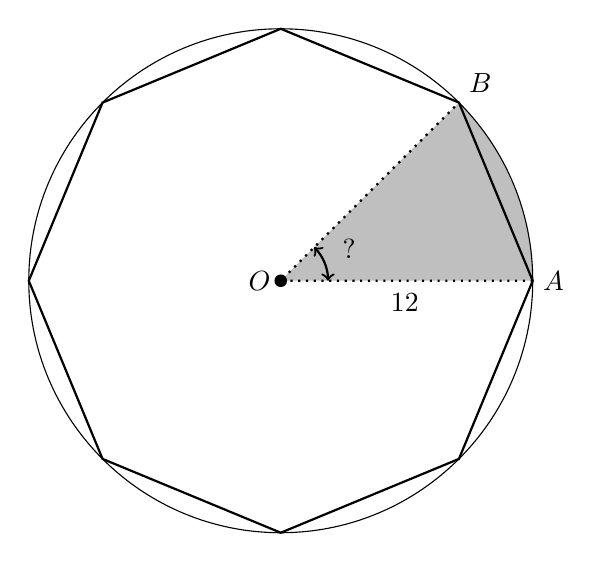
\begin{tikzpicture}[scale=0.8]
    \fill [lightgray]
    (0,0)--(0:4) arc (0:45:4)--(0,0);
    \draw (0,0) circle[radius=4];
    \draw [thick, <->] (0:0.75) arc (0:45:0.75);
    \draw [thick, dotted]
    (0:4) node[right] {$A$}--
    (0,0) node[left] {$O$}--
    (45:4) node[above right] {$B$};
    \draw [thick]
    (0:4)--(45:4)--(90:4)--(135:4)--(180:4)--(225:4)--(270:4)--(315:4)--cycle;
    \fill (0,0) circle[radius=.1];
    \node at (25:1.2) {$?$};
    \node at (-10:2) {$12$};
  \end{tikzpicture}
  \end{multicols}

\newpage
\item Given circle $O$ with $m \wideparen{AB}=68^\circ$.
  \begin{multicols}{2}
    \raggedcolumns
    \begin{enumerate}
      \item Write down the $m\angle AOB$. \vspace{1.7cm}
      \item Find the $m\angle ACB$. \vspace{2cm}
    \end{enumerate}
      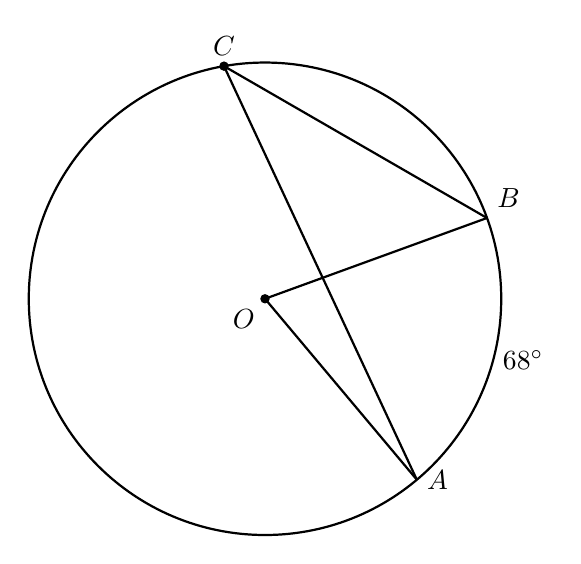
\begin{tikzpicture}[scale=.6, rotate=-90]
        \draw [thick] (0,0) circle[radius=5];
        \fill (0,0) circle[radius=.1];
        \draw [thick]
        (40:5) node[right] {$A$}--
        (0,0) node[below left] {$O$}--
        (110:5) node[above right] {$B$};
        \draw [thick] (40:5)--(190:5) node[above] {$C$}--(110:5);
        \fill (190:5) circle[radius=.1];
        \draw (75:5) node[right]{$68^\circ$};
      \end{tikzpicture}
  \end{multicols}
  
\newpage
\item A circle on the coordinate plane has center $C$ and radius $\overline {CT}$. A tangent line through point $T$ is drawn, as shown.
\begin{multicols}{2}
  \begin{enumerate}[itemsep=1.25cm]
    \item Write down the center of the circle as a coordinate pair.
    \item Write down the equation of the circle.
    \item What is the slope of the radius $\overline {CT}$?
    \item Find the slope of the tangent line.
  \end{enumerate}
    \vspace{2cm}
    \begin{flushright}
    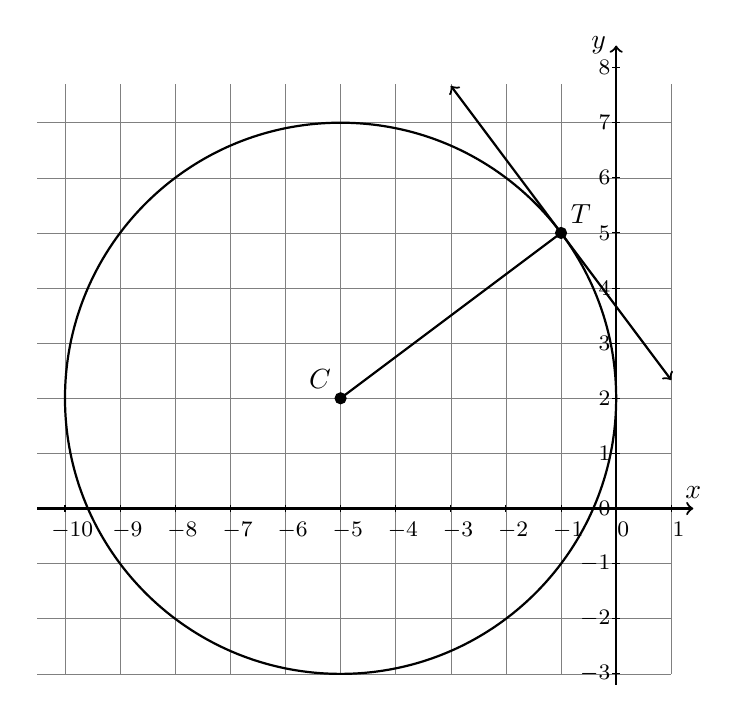
\begin{tikzpicture}[scale=0.7]
      \draw [help lines] (-10.5,-3) grid (1,7.7);
      \draw [thick, ->] (-10.5,0) -- (1.4,0) node [above] {$x$};
      \foreach \x in {-10,-9,...,1}
        \draw[shift={(\x,0)},color=black] (0pt,2pt) -- (0pt,-2pt) node[below] {\footnotesize \; $\x$};
      \draw [thick, ->] (0,-3.2)--(0,8.4) node [left] {$y$};
      \foreach \y in {-3,-2,...,8}
        \draw[shift={(0,\y)},color=black] (-2pt,0pt) -- (2pt,0pt) node[left] {\footnotesize \; $\y$};
      \draw [thick] (-5,2) circle [radius=5];
      \draw [fill] (-5,2) circle [radius=0.1] node[above left] {$C$};
      \draw [fill] (-1,5) circle [radius=0.1] node[above right] {$T$};
      \draw [-, thick] (-5,2)--(-1,5);
      \draw [<->, thick] (-3,7.67)--(1,2.33);
    \end{tikzpicture}
    \end{flushright}
\end{multicols}

\newpage
\item Two supplementary angles have measures $m\angle ABD = 8x$ and $m\angle DBC = 11x + 56.5^\circ$. \\[0.25cm] 
Write an equation applying the angle addition theorem, then find $x$. \vspace{0.5cm}
  \begin{flushright}
    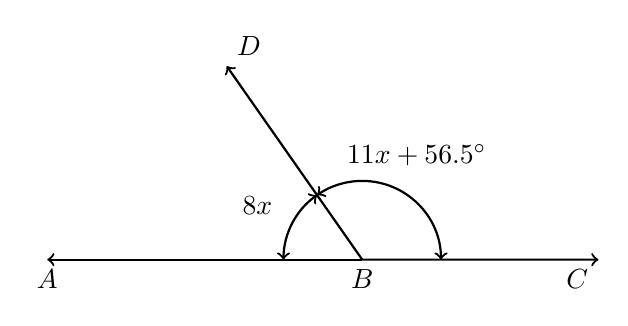
\begin{tikzpicture}[scale=1]
      \draw [<->, thick]
        (0:3) coordinate (a) node[below left] {$C$}
        -- (0,0) coordinate (b) node[below] {$B$}
        -- (125:3) coordinate (c) node[above right] {$D$}
        pic["$11x+56.5^\circ$", <->, draw=black, angle eccentricity=1.5, angle radius=1cm]
        {angle=a--b--c};
        \draw [<-, thick]
        (180:4) coordinate (d) node[below] {$A$}
        -- (0,0) coordinate (e)
        pic["$8x$", <->, draw=black, angle eccentricity=1.5, angle radius=1cm]
        {angle=c--e--d};
    \end{tikzpicture}
  \end{flushright}
  %https://graspablemath.com/canvas?load=_324d9aa72a142273

\newpage
\item Given circle with center $I$ and $m\angle TIP=82^\circ$. Find the measure of each arc or angle.
  \begin{multicols}{2}
    \raggedcolumns
    \begin{enumerate}[itemsep=1cm]
      \item $m \wideparen{TP}$
      \item $m\angle TAP$
      \item $m\angle API$
      \item $m\angle PIA$
    \end{enumerate}
      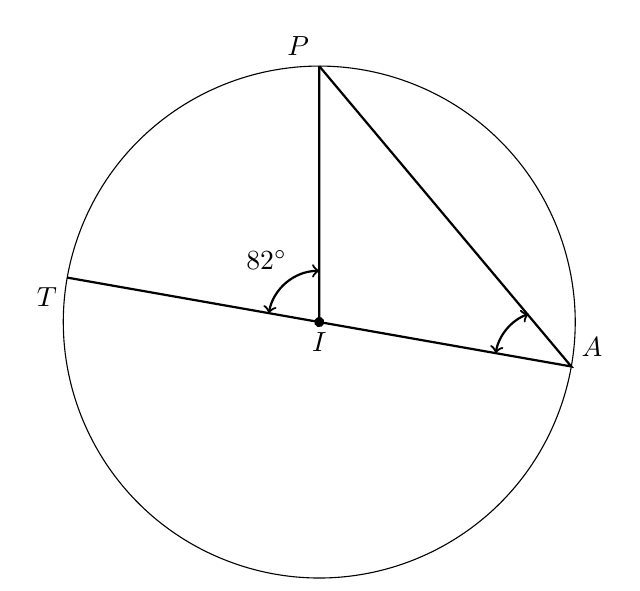
\begin{tikzpicture}[scale=.65, rotate=-20]
        \draw (0,0) circle[radius=5];
        \fill (0,0) circle[radius=.1];
        \draw [thick]
        (190:5) node[below left] {$T$}--
        (0,0) node[below] {$I$}--
        (110:5) node[above left] {$P$};
        \draw [thick] (0,0)--(10:5) node[above right] {$A$}--(110:5);
        \draw (130:1.3) node[left]{$82^\circ$};
        \draw [thick, <->] (110:1) arc (110:190:1);
        \draw [thick, <->] (10:3.5) arc (190:130:1);
      \end{tikzpicture}
  \end{multicols}

\newpage
\item What is the equation of a circle with center $(1,-3)$ and radius $r=2$?\\[0.5cm]
  Graph the circle in Graspable Math or Geogebra and paste the image here.
  %https://graspablemath.com/canvas?load=_6a89b545540e2be5

\newpage
\item Line segment $\overline{AB}$, $A(1,8)$, $B(9,2)$, is the diameter of circle $M$. 
\begin{enumerate}
  \item On the grid, mark and label as a coordinate pair the midpoint of the segment, the circle center $M$. 
  \item Calculate the length of $\overline{AB}$ and hence, the radius of the circle.\
  \item Write down the equation of the circle. 
  \item Sketch the circle on the grid or draw it with Geogebra or Graspable Math.
\end{enumerate}
\begin{flushright}
  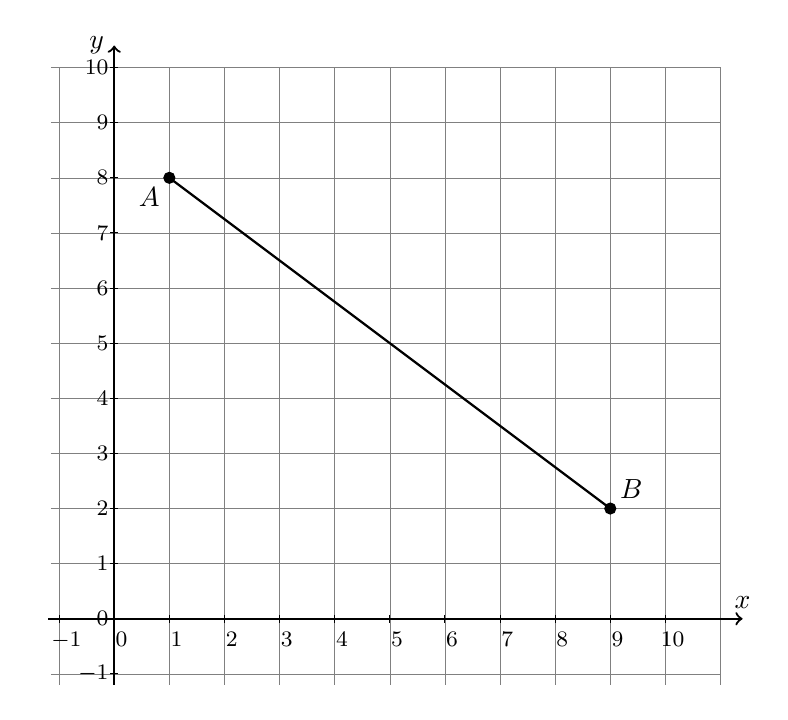
\begin{tikzpicture}[scale=0.7]
    \draw [help lines] (-1.15,-1.2) grid (11,10);
    \draw [thick, ->] (-1.2,0) -- (11.4,0) node [above] {$x$};
    \foreach \x in {-1,0,...,10}
      \draw[shift={(\x,0)},color=black] (0pt,2pt) -- (0pt,-2pt) node[below] {\footnotesize \; $\x$};
    \draw [thick, ->] (0,-1.2)--(0,10.4) node [left] {$y$};
    \foreach \y in {-1,0,1,...,9, 10}
      \draw[shift={(0,\y)},color=black] (-2pt,0pt) -- (2pt,0pt) node[left] {\footnotesize \; $\y$};
    %\draw [thick] (6,3) circle [radius=5];
    \draw [fill] (1,8) circle [radius=0.1] node[below left] {$A$};
    \draw [fill] (9,2) circle [radius=0.1] node[above right] {$B$};
    \draw [-, thick] (1,8)--(9,2);
    %\draw [<->, thick] (-0.6,4.3)--(5,8.5);
  \end{tikzpicture}
  \end{flushright}
  %https://graspablemath.com/canvas?load=_024bda2a5587c074
  %https://graspablemath.com/canvas?load=_6a89b545540e2be5

\end{enumerate}
\end{document}